% !TeX root = ../thesis.tex

%%%%%%%%%%%%%%%%%%%%%%%%%%%%%%%%%%%%%
\thesischapter[ch:community][0.7\textwidth]
  {``The whole is something else than the sum of its parts.''}
  {--- Kurt Koffka, 1935}
  {Community-level summaries}
\nocite{koffka1935principles}
\chapterabstract{This chapter introduces the first of the three analysis target levels considered in this thesis: community-level summaries. Rather than focusing on individual taxa or pairwise associations, these methods reduce characteristic properties of the microbial community to interpretable summary quantities, either at the level of a single sample or for an entire population. Within-sample diversity, between-sample dissimilarity, community dispersion, regression for compositional responses, and compositional equivalence provide complementary views on global microbiome variation. The chapter establishes the methodological foundation for the community-level part of the integrated analysis in Chapter~\ref{ch:application}.}
\chaptercontents
%%%%%%%%%%%%%%%%%%%%%%%%%%%%%%%%%%%%%

%%%%%%%%%%%%%%%%%%%%%%%%%%%%%%%%%%%%%
\section{Introduction}
\label{sec:3community:intro}
%%%%%%%%%%%%%%%%%%%%%%%%%%%%%%%%%%%%%

This chapter considers community-level analyses, in which the microbial community is summarized or modeled as a whole rather than through individual taxa or pairwise associations. Such analyses provide complementary perspectives on global community structure and are often used to assess whether microbial communities differ across samples, groups, or environmental conditions.

Community-level approaches can be distinguished by the statistical object they summarize. Within-sample diversity measures, commonly referred to as alpha diversity, reduce each sample to a scalar quantity describing characteristics such as richness, evenness, or dominance. Between-sample dissimilarities, often discussed under the term beta diversity, quantify differences between pairs of samples and thereby represent the structure of an entire sample collection through a distance or dissimilarity matrix. These dissimilarities form the basis for ordination, distance-based group comparisons such as PERMANOVA, and analyses of community dispersion. A further perspective is provided by regression models for compositional responses, in which the transformed microbial composition is modeled directly as a multivariate outcome. Finally, compositional equivalence testing addresses a complementary inferential question by assessing whether group differences are sufficiently small to be regarded as practically negligible.

The appropriate representation of the data depends on the method under consideration. As discussed in Chapter~\ref{ch:microbiome}, microbiome count data are compositional, sparse, and characterized by heterogeneous library sizes. Some community-level methods, such as model-based richness estimation, are designed to account for unequal sampling depth and uncertainty due to unobserved taxa and can therefore operate directly on count data. Other approaches require a transformation or dissimilarity measure that is compatible with the relative nature of the observations. These choices determine the statistical object under study and consequently affect the interpretation of diversity estimates, distances, regression coefficients, and group comparisons.

The chapter is organized into four parts. Section~\ref{sec:3community:within_sample_div} introduces within-sample diversity measures, including richness, Shannon diversity, and Gini--Simpson diversity, together with methods for group comparison and regression modeling. Section~\ref{sec:3community:between_sample_diss} considers between-sample dissimilarities, with particular emphasis on Bray--Curtis dissimilarity and Euclidean distance after centered log-ratio transformation. These quantities are subsequently used for ordination, PERMANOVA, and the assessment of group differences in multivariate dispersion. Section~\ref{sec:3community:regression} discusses regression models for compositional responses, whereas Section~\ref{sec:3community:compositional_equivalence} introduces compositional equivalence testing as an alternative to conventional difference testing.

Together, these methods characterize community structure at complementary resolutions: within-sample diversity summarizes individual samples, between-sample dissimilarities describe relationships among samples, compositional-response regression relates covariates to the community profile, and equivalence testing evaluates whether group-level compositional differences are practically small. They form the community-level component of the integrated analysis in Chapter~\ref{ch:application}.


%%%%%%%%%%%%%%%%%%%%%%%%%%%%%%%%%%%%%
\section{Within-sample diversity}
\label{sec:3community:within_sample_div}
%%%%%%%%%%%%%%%%%%%%%%%%%%%%%%%%%%%%%

\begin{figure}[H]
\centering
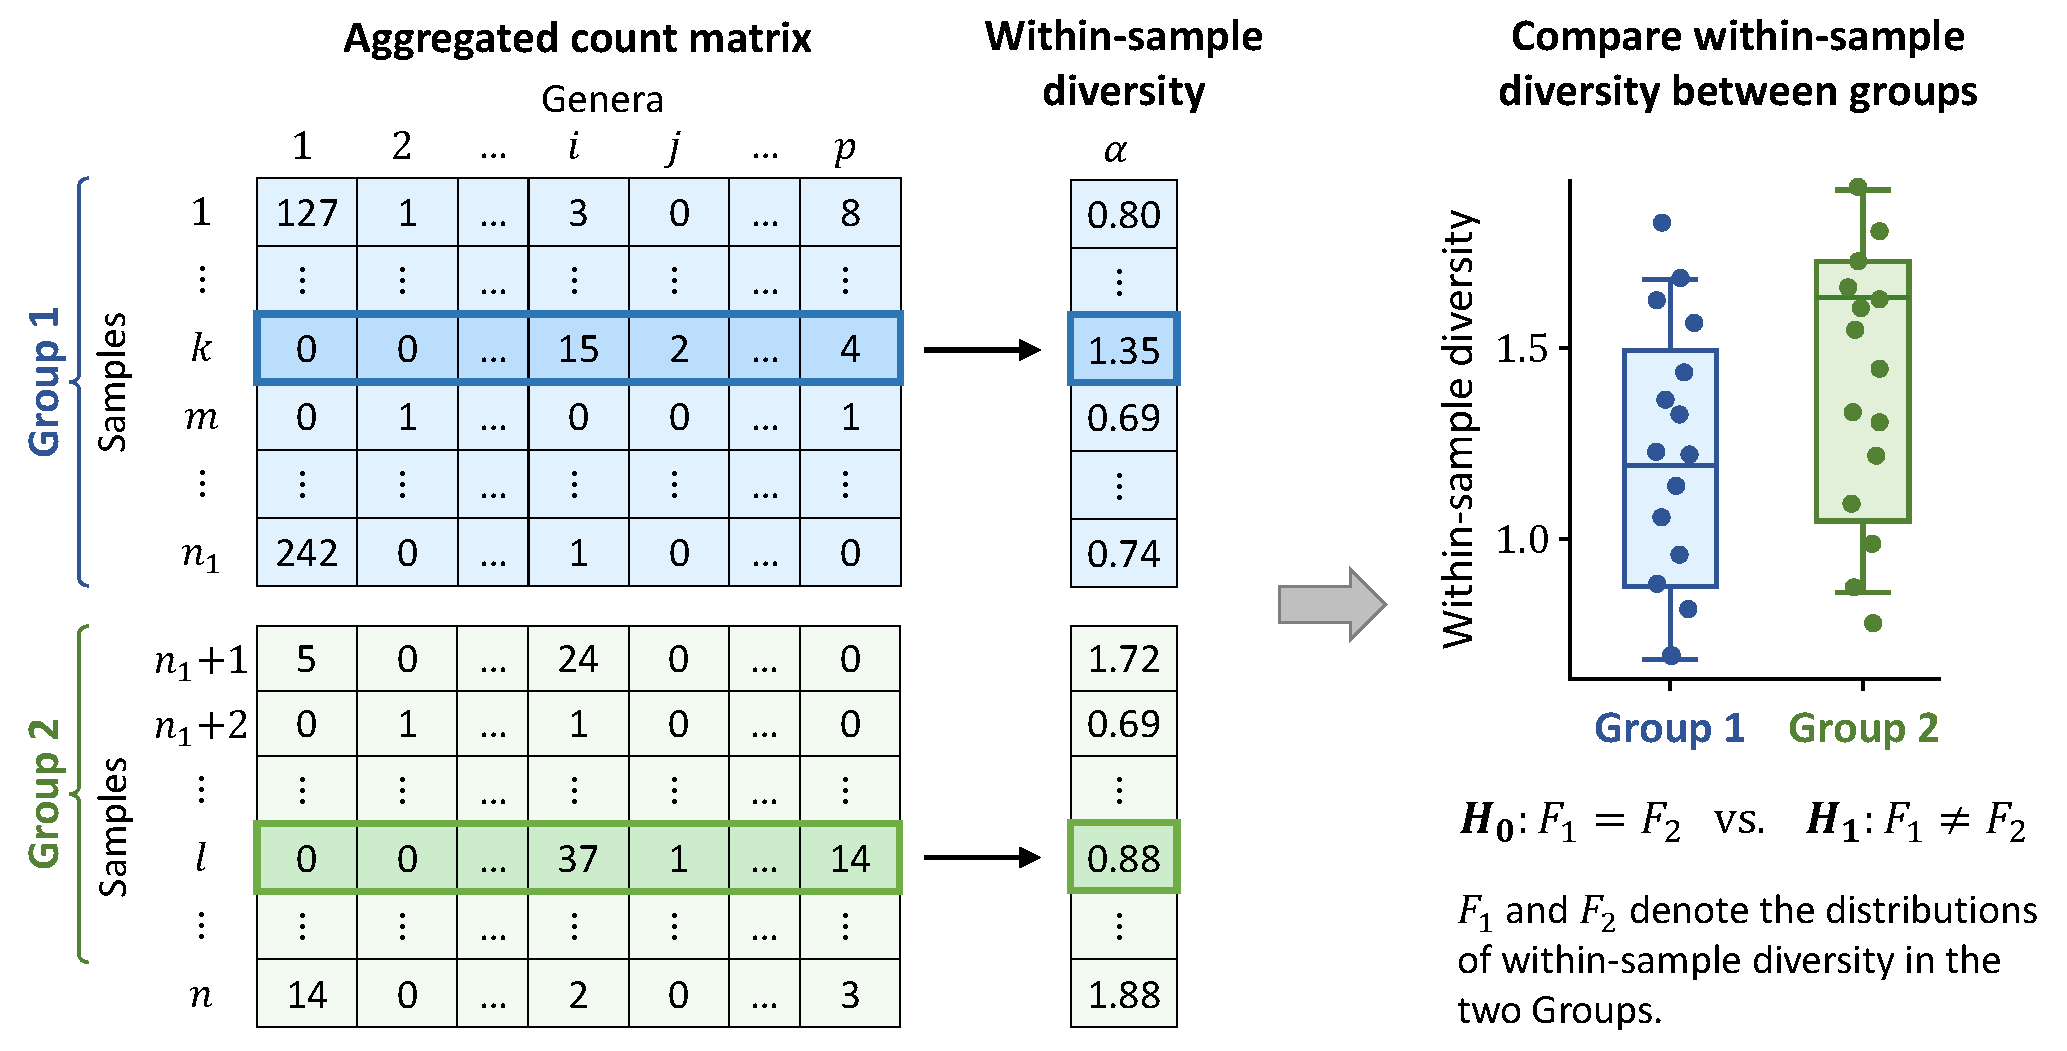
\includegraphics[width=\textwidth]{../ch03_community_level/overview_figures/overview_alpha.pdf}
\caption{\textbf{Overview of within-sample diversity analysis.} The unfiltered taxonomically aggregated count matrix, with samples in rows and taxa in columns, serves as the input for within-sample diversity analysis. Summarizing counts across taxa yields one diversity value per sample, for example an alpha-diversity measure. These sample-level values can then be compared between groups using parametric or non-parametric tests.}
\label{fig:3community:overview_alpha_diversity}
\end{figure}

Within-sample diversity, commonly referred to as \emph{alpha diversity}, describes the diversity of the microbial community observed within an individual sample. Alpha diversity measures reduce the high-dimensional taxonomic composition of each sample to a scalar quantity and therefore represent community-level summaries in the framework of analysis targets introduced in Chapter~\ref{ch:introduction}. Because they yield one value per sample, these measures are widely used in exploratory analyses, group comparisons, and regression settings, where the diversity estimate serves as the response variable.

Different alpha diversity measures emphasize different aspects of within-sample community structure. Richness measures quantify the number of taxa present, whereas diversity indices additionally account for the distribution of abundances across taxa. The Shannon index and the Gini--Simpson index are examples of such entropy- and dominance-based indices, respectively. As discussed in Chapter~\ref{ch:microbiome}, microbiome data are characterized by finite and heterogeneous sampling depth, sparsity, and a large proportion of rare taxa. These features have important implications for the estimation and comparison of alpha diversity, in particular for richness, which is sensitive to unobserved taxa and sampling effort.

To address these challenges, we focus on model-based approaches to diversity estimation that explicitly account for unequal sampling depth and the presence of unobserved taxa. In particular, we consider richness estimation via the \texttt{breakaway} framework and entropy-based diversity estimation using \texttt{DivNet}. These methods provide estimates together with uncertainty measures, which enables statistical comparison and regression modeling without relying on procedures such as rarefaction that modify the observed count matrix.

In the following, we first introduce richness estimation and then discuss diversity indices that incorporate abundance distributions. We then describe approaches for statistical comparison and regression modeling based on these sample-level community summaries. Figure~\ref{fig:3community:overview_alpha_diversity} provides a schematic overview of the workflow for estimating and comparing within-sample diversity across groups.


%====================================
\subsection{Richness estimation}
\label{sec:3community:within:richness}
%====================================

Richness is a basic measure of alpha diversity and is defined as the number of distinct taxa present in a sample. In the context of microbiome data, richness aims to quantify how many microbial features, such as amplicon sequence variants (ASVs), are represented in a community. Formally, for a sample $k$, the observed richness is given by
\begin{equation}
\alpha_{\mathrm{rich}, k}^{\mathrm{obs}} = \sum_{i=1}^p \mathbb{I}(x_{ki} > 0),
\end{equation}
where $\mathbb{I}(\cdot)$ denotes the indicator function. However, under incomplete sampling, the observed number of taxa typically underestimates the richness of the underlying community because low-abundance taxa may remain unobserved.

As discussed in Chapter~\ref{ch:microbiome}, microbiome data are characterized by high sparsity and a large proportion of rare taxa. Many taxa occur at low abundance and may not be observed in all samples, particularly when sequencing depth is limited. As a result, the naive richness estimator tends to underestimate the true richness, and comparisons across samples are confounded by differences in sampling effort.

To address these challenges, we focus on approaches to diversity estimation that account for unequal sampling depth and the presence of unobserved taxa. As discussed in Section~\ref{sec:2micro:norm:rarefaction}, rarefaction provides a simple and widely used strategy to equalize library sizes by subsampling counts to a common depth, and is often employed in diversity and distance-based analyses. However, rarefaction achieves comparability by discarding observed counts and therefore comes at the cost of information loss, which is particularly consequential for richness estimation where rare taxa play a central role.

An alternative approach is proposed by \citet{willis2015estimating}, who estimate the number of unobserved taxa rather than reducing the observed data through subsampling. In particular, we consider richness estimation via the \texttt{breakaway} framework and entropy-based diversity measures estimated with \texttt{DivNet}. These methods provide model-based estimates and associated uncertainty measures, facilitating comparisons of diversity across samples and groups without relying on rarefaction. Conceptually, this shifts the treatment of heterogeneous sampling depth from a preprocessing step to an explicit component of the statistical model, where uncertainty due to incomplete sampling is directly accounted for in the estimation.

For a given sample $k$, let $n_j^{(k)}$ denote the number of taxa observed exactly $j$ times, that is,
\begin{equation}
n_j^{(k)} = \#\{i : x_{ki} = j\}.
\end{equation}
The total richness can then be written as
\begin{equation}
\alpha_{\mathrm{rich}, k} = \sum_{j \geq 0} n_j^{(k)},
\end{equation}
where $n_0^{(k)}$ denotes the number of unobserved taxa. The estimation problem therefore reduces to predicting $n_0^{(k)}$. Here, the notion of an unobserved taxon is defined relative to the feature universe represented by the sequencing and preprocessing workflow, not to all microbial taxa that could in principle occur in the sampled environment.

The approach of \citet{willis2015estimating} models the ratios of adjacent frequency counts,
\begin{equation}
\frac{n_{j+1}^{(k)}}{n_j^{(k)}},
\end{equation}
as a function of $j$, motivated by classical characterizations of discrete distributions via adjacent probability ratios. In particular, a broad class of distributions can be represented through probability ratios that take the form of rational functions in $j$, providing a flexible modeling framework beyond traditional assumptions such as mixed Poisson models. A nonlinear regression model is fitted to the observed ratios, accounting for their sampling variability through appropriate weighting, and subsequently extrapolated to $j = 0$ to estimate the ratio $n_1^{(k)} / n_0^{(k)}$, from which the number of unobserved taxa is obtained. The resulting richness estimate is given by
\begin{equation}
\hat{\alpha}_{\mathrm{rich}, k} = \sum_{j \geq 1} n_j^{(k)} + \hat{n}_0^{(k)}.
\end{equation}

The \texttt{breakaway} R package provides a practical implementation of this framework using a finite set of low-order ratio models, weighted nonlinear least squares fitting, and a data-driven model selection procedure. Standard errors are obtained via a delta-method approximation. Compared to naive richness estimates, this approach explicitly accounts for rare and unobserved taxa and does not require rarefaction, as differences in sampling depth are incorporated into the modeling framework.

%====================================
\subsection{Diversity indices}
\label{sec:3community:within:diversity}
%====================================

In addition to richness, alpha diversity measures often incorporate information on the relative abundances of taxa within a community. While richness quantifies the number of distinct taxa present, it treats all taxa equally and ignores how sequencing counts are distributed among them. As a result, two communities with the same richness may differ substantially in their ecological structure, for example if one is dominated by a few highly abundant taxa while the other exhibits a more even distribution. Such differences are particularly relevant in microbiome studies, where communities are typically characterized by a small number of dominant taxa and a long tail of low-abundance taxa. Therefore, diversity measures that account for relative abundances provide a more informative summary of community structure beyond mere presence or absence.

Let $z_{ki} \in [0,1]$ denote the (unknown) relative abundance of taxon $i$ in sample $k$, such that $\sum_{i=1}^p z_{ki} = 1$. The Shannon entropy is defined as
\begin{equation}
\label{eq:3community:shannon}
\alpha_{\mathrm{Sh}, k} = - \sum_{i=1}^p z_{ki} \log(z_{ki}),
\end{equation}
and captures both richness and evenness of the community \citep{willis2018divnet}. For a fixed number of taxa, the Shannon index is maximized when all taxa are equally abundant and decreases as the distribution becomes more uneven. In particular, it places relatively high weight on low-abundance taxa.

Following \citet{willis2018divnet}, the Simpson index is defined as
\begin{equation}
\label{eq:3community:simpson}
\alpha_{\mathrm{Si}, k} = \sum_{i=1}^p z_{ki}^2.
\end{equation}
It can be interpreted as the probability that two randomly drawn individuals from the community belong to the same taxon. In contrast to the Shannon entropy, the Simpson index is less sensitive to rare taxa and primarily reflects dominance structure within the community.

In practice, the relative abundances $z_{ki}$ are not directly observed. A common approach is to estimate them by empirical proportions,
\begin{equation}
\hat{z}_{ki}^{\mathrm{plug-in}} = \frac{x_{ki}}{m_k},
\end{equation}
yielding plug-in estimators of the diversity indices. However, such estimators are known to be biased, particularly in the presence of sparse data and unobserved taxa, which are common in microbiome studies \citep{willis2018divnet}.

To address these limitations, \citet{willis2018divnet} proposed \texttt{DivNet}, which estimates diversity indices based on a model for the underlying compositional structure of the data. The methodology is implemented in the \texttt{DivNet} R package, which provides functions for model fitting, diversity estimation, and uncertainty quantification. Rather than treating samples independently, \texttt{DivNet} models log-ratios of relative abundances across samples using a multivariate normal distribution, thereby accounting for covariance in the log-ratio representation and borrowing strength across samples.

More specifically, let $\mathbf{z}_k \in \mathcal{S}^{p-1}$ denote the latent relative abundance vector for sample~$k$. \texttt{DivNet} assumes that log-ratios of $\mathbf{z}_k$ follow a multivariate normal model with mean depending on covariates and covariance capturing dependence between taxa. Based on the fitted model, an estimate $\hat{\mathbf{z}}_k$ of the latent composition is obtained. The diversity indices are then evaluated by substituting $\hat{z}_{ki}$ into Equations~\eqref{eq:3community:shannon} and~\eqref{eq:3community:simpson}.

A key advantage of this approach is that it estimates diversity at the level of the underlying compositional structure rather than directly from the observed counts, allowing information to be shared across samples and improving estimation accuracy, especially in high-dimensional and sparse settings. Furthermore, by modeling log-ratio transformed abundances jointly across taxa, the approach accounts for dependence structures that are ignored by plug-in estimators.

%====================================
\subsection{Testing within-sample diversity}
\label{sec:3community:within:testing}
%====================================

The diversity measures introduced above yield one scalar value per sample and can therefore be analyzed using standard statistical methods for scalar outcomes. In the context of group comparisons, the primary objective is to assess whether diversity differs across levels of a categorical covariate.

A commonly used nonparametric approach is the Kruskal--Wallis test, which evaluates the null hypothesis
\begin{equation}
H_0: F_1 = F_2 = \cdots = F_G,
\end{equation}
where $F_g$ denotes the distribution of the diversity measure in group $g = 1,\dots,G$. In the case of two groups, this reduces to the Wilcoxon rank-sum test. These tests are based on rank statistics and rely on asymptotic approximations for significance assessment.

As an alternative, permutation-based tests provide a flexible framework that does not rely on distributional assumptions. Let $\hat{\alpha}_k$ denote a diversity estimate for sample $k$, and let $g_k \in \{1,\dots,G\}$ denote the corresponding group label. A test statistic $T = T(\{\hat{\alpha}_k, g_k\}_{k=1}^n)$ is computed for the observed data, for example the Kruskal-Wallis statistic or a difference in group means or medians. Under the null hypothesis and an exchangeable study design, the labels $g_k$ can be permuted to approximate the null distribution of $T$. The corresponding empirical $p$-value is given by
\begin{equation}
p_{\mathrm{emp}} = \frac{1 + \sum_{b=1}^B \mathbb{I}(T_b^* \geq T_{\mathrm{obs}})}{1 + B},
\end{equation}
where $T_{\mathrm{obs}}$ denotes the observed test statistic and $T_b^*$ the statistic obtained from the $b$-th permutation.

As discussed in Chapter~\ref{ch:permapprox}, empirical $p$-values lie on a coarse grid when only a limited number of permutations $B$ can be performed. In the present setting, this limitation is often less critical because alpha diversity analysis usually involves only one or a small number of tests, so that the multiplicity burden is substantially smaller than in high-dimensional feature-level analyses. In contrast to high-dimensional settings with many simultaneous tests, the coarse resolution of empirical $p$-values therefore has limited impact on inference. However, if a finer resolution of $p$-values is desired without substantially increasing the number of permutations, the empirical permutation distribution can be refined by tail approximation methods such as the approach implemented in \texttt{permApprox} (Chapter~\ref{ch:permapprox}).


%====================================
\subsection{Regression modeling of within-sample diversity}
\label{sec:3community:within:regression}
%====================================

\begin{figure}[H]
	\centering
	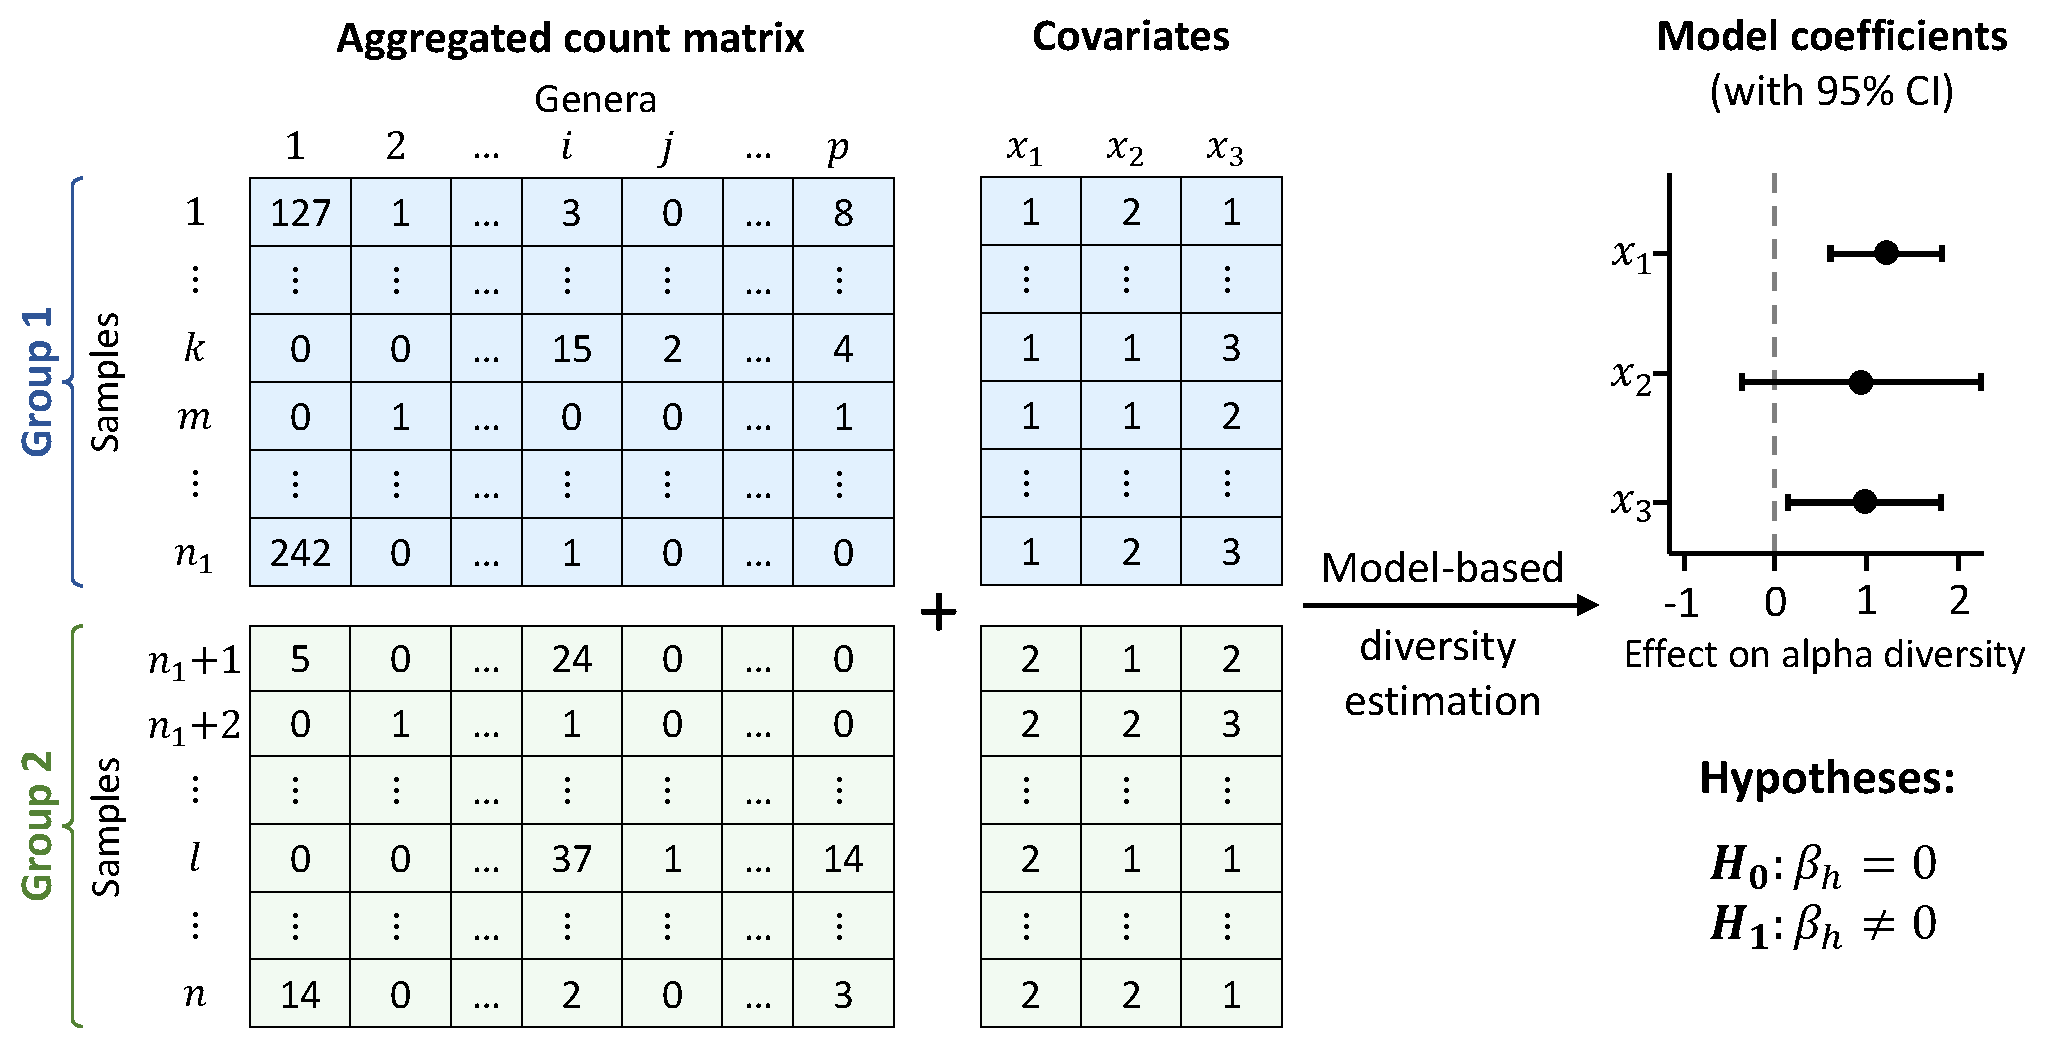
\includegraphics[width=\textwidth]{../ch03_community_level/overview_figures/overview_divnet.pdf}
	\caption{\textbf{Overview of regression-based within-sample diversity analysis.} The unfiltered taxonomically aggregated count matrix and sample-level covariates serve as input for model-based diversity estimation and regression. Methods such as \texttt{breakaway} and \texttt{DivNet} estimate within-sample diversity while accounting for incomplete sampling and, in the case of \texttt{DivNet}, covariance in the log-ratio representation across samples. The resulting regression coefficients quantify associations between covariates and the underlying diversity parameter and can be accompanied by confidence intervals and hypothesis tests.}
	\label{fig:3community:overview_divnet}
\end{figure}

Beyond group comparisons, alpha diversity measures can be analyzed within a regression framework to assess associations with covariates and to adjust for potential confounding factors. In this setting, the diversity measure serves as a response variable, while explanatory variables may include clinical, environmental, or technical factors.

A straightforward approach is to treat the estimated diversity values $\hat{\alpha}_k$ as observed responses and apply standard regression models. Let $\hat{\alpha}_k$ denote the estimated alpha diversity for sample $k$, and let $\mathbf{x}_k$ be a vector of covariates. A simple linear regression model is then given by
\begin{equation}
\hat{\alpha}_k = \beta_0 + \mathbf{x}_k^\top \boldsymbol{\beta} + \varepsilon_k,
\end{equation}
where $\boldsymbol{\beta}$ are regression coefficients and $\varepsilon_k$ is an error term with conditional mean zero given the covariates. Inference is typically based on testing hypotheses of the form $H_0:\beta_h = 0$, where $h$ indexes the covariates, corresponding to the absence of an association between the covariate $x_{kh}$ and the diversity measure.

While this approach is easy to implement and widely used in practice, it implicitly treats the diversity estimates as error-free observations. However, as discussed above, alpha diversity measures are themselves estimated quantities and may exhibit substantial uncertainty, particularly in the presence of sparse data and unobserved taxa.

To account for this, a more principled approach is provided by the model-based framework of \citet{willis2017improved}, which incorporates estimation uncertainty directly into the regression model. Let $\hat{\alpha}_k$ denote a diversity estimate together with its estimated standard error. The model assumes
\begin{equation}
\hat{\alpha}_k = \beta_0 + \mathbf{x}_k^\top \boldsymbol{\beta} + u_k + \varepsilon_k,
\end{equation}
where $u_k$ captures biological variability between samples and $\varepsilon_k$ represents estimation error, whose variance is assumed to be known or estimated from the diversity estimation procedure. Inference is again based on hypotheses of the form $H_0: \beta_h = 0$, with the regression model targeting the underlying diversity parameter while accounting for uncertainty in its estimated sample-level values.

This framework, originally developed for richness estimation, applies more generally to diversity measures for which standard errors are available. In particular, it can be combined with richness estimates obtained via \texttt{breakaway} as well as entropy-based diversity measures estimated using \texttt{DivNet}. The resulting procedure is implemented in the \texttt{breakaway} R package via the \texttt{betta} function. A schematic overview of this model-based regression framework is shown in Figure~\ref{fig:3community:overview_divnet}.

In contrast to the naive regression model, which ignores estimation uncertainty, the model-based approach separates biological variability from measurement error and can lead to more reliable inference when diversity estimates are noisy. However, it relies on additional assumptions, including approximate normality of the diversity estimates and accurate estimation of their standard errors.



%%%%%%%%%%%%%%%%%%%%%%%%%%%%%%%%%%%%%
\section{Between-sample dissimilarity}
\label{sec:3community:between_sample_diss}
%%%%%%%%%%%%%%%%%%%%%%%%%%%%%%%%%%%%%

Within-sample diversity, as introduced in the previous section, summarizes each microbial community by one scalar quantity per sample. Many questions in microbiome analysis, however, concern how microbial communities differ \emph{between} samples. This complementary perspective is based on pairwise comparisons of taxon profiles and leads to an $n \times n$ dissimilarity matrix rather than to a single value per sample. Figure~\ref{fig:3community:overview_beta_diversity} illustrates this general workflow. In the following, we first introduce between-sample dissimilarities as community-level summaries and clarify their relationship to the ecological concept of beta diversity. We then discuss two commonly used choices of dissimilarity, Bray--Curtis dissimilarity and Euclidean distance after log-ratio transformation, before turning to ordination, PERMANOVA, and tests for differences in community dispersion.

\begin{figure}[H]
	\centering
	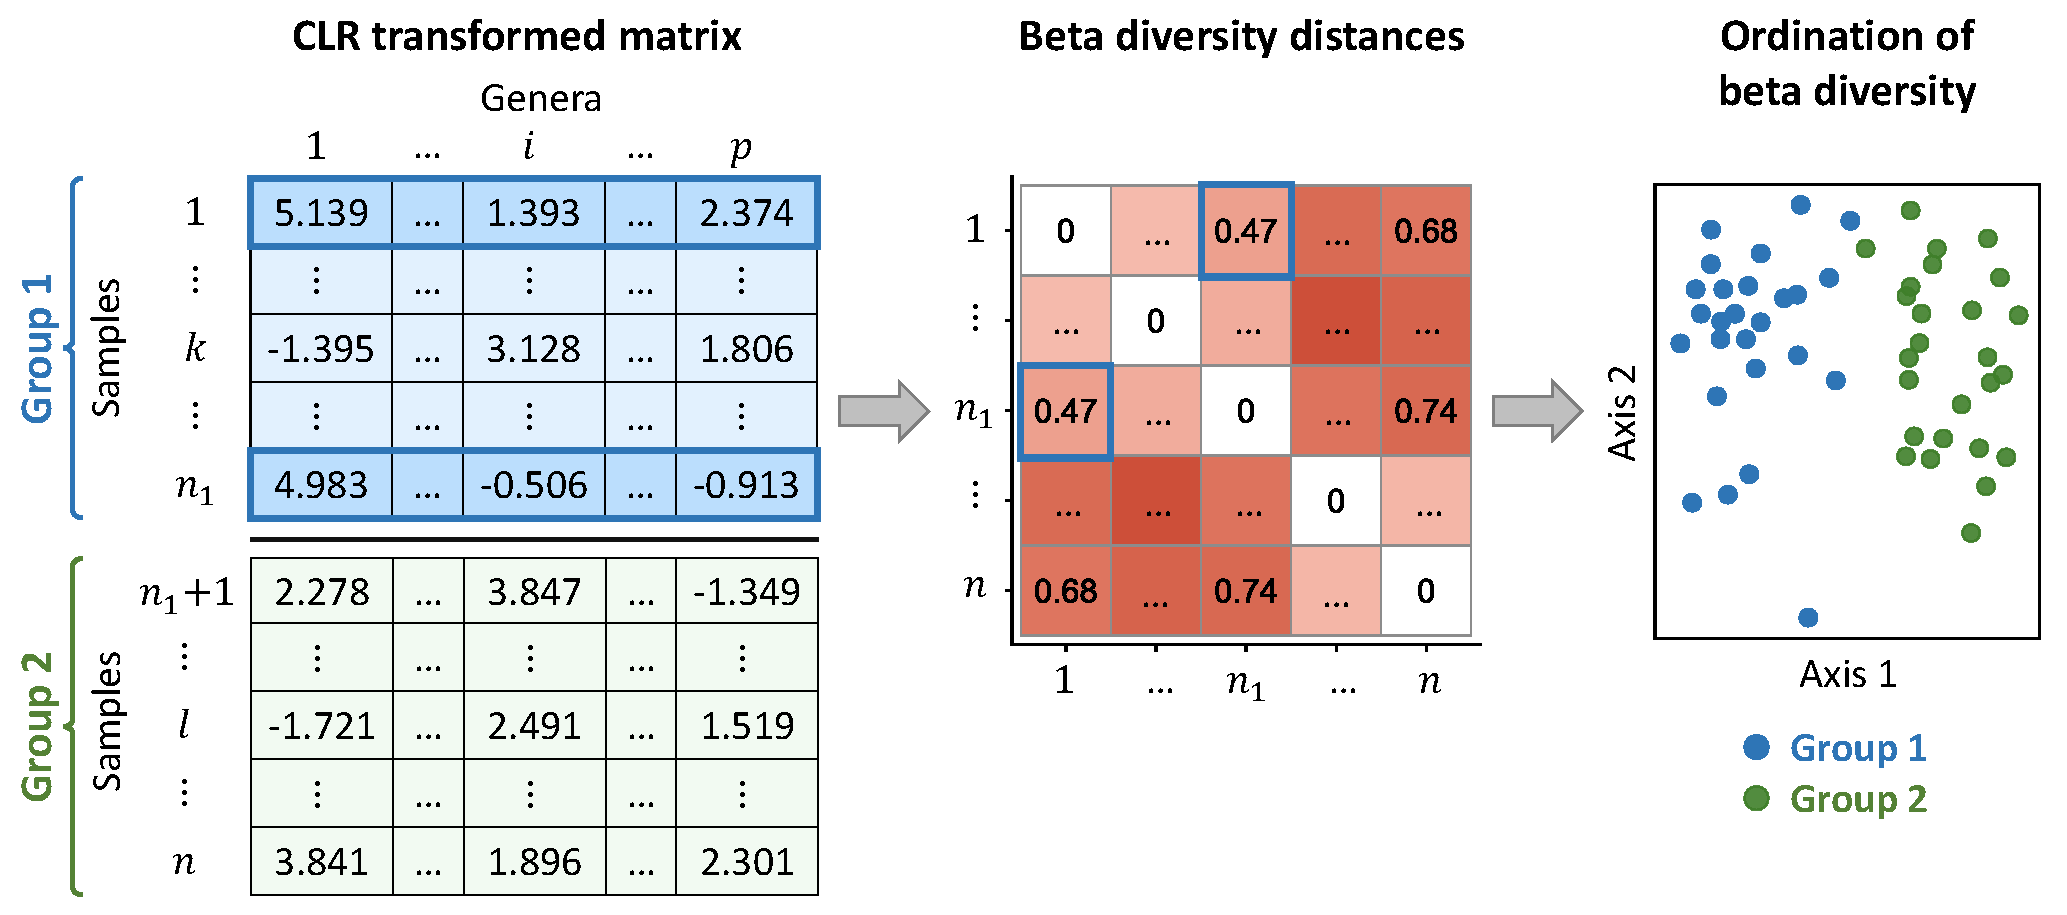
\includegraphics[width=\textwidth]{../ch03_community_level/overview_figures/overview_beta.pdf}
	\caption{\textbf{Overview of between-sample diversity analysis.} After zero handling and CLR transformation, the transformed count matrix is represented by a sample-by-sample distance matrix, here, Euclidean distances between CLR coordinates correspond to Aitchison distances. The resulting beta-diversity distances quantify compositional dissimilarity between samples and can be explored by ordination or used for distance-based group comparisons such as PERMANOVA and PERMDISP.}
	\label{fig:3community:overview_beta_diversity}
\end{figure}

%====================================
\subsection{Beta diversity as a dissimilarity-based summary}
\label{sec:3community:between:beta}
%====================================

In ecology, \emph{beta diversity} describes variation in community composition among sampling units \citep{whittaker1960vegetation,anderson2011navigating}. Since microbiome data also represent communities of co-occurring organisms observed across samples, the same conceptual framework is commonly applied in microbiome studies. In practice, beta diversity is typically represented through pairwise dissimilarities between samples. In this thesis, we use the term between-sample dissimilarity when referring to the statistical object underlying these analyses, namely a pairwise matrix derived from the taxon profiles of all samples.

Let $\mathbf{x}_k=(x_{k1},\ldots,x_{kp})^\top$ and $\mathbf{x}_l=(x_{l1},\ldots,x_{lp})^\top$ denote the taxon profiles of two samples $k$ and $l$. A dissimilarity or distance function $d(\cdot,\cdot)$ assigns a non-negative value $d(\mathbf{x}_k,\mathbf{x}_l)$ to this pair, where smaller values indicate more similar microbial communities and larger values indicate stronger differences. Applying $d$ to all sample pairs yields an $n \times n$ dissimilarity matrix $\mathbf{D}=(d_{kl})$, with entries $d_{kl}=d(\mathbf{x}_k,\mathbf{x}_l)$. For the measures considered here, $\mathbf{D}$ is symmetric and has zeros on the diagonal.

The matrix $\mathbf{D}$ is a community-level summary because each entry aggregates information across all taxa in the two samples being compared. It retains information about which samples are similar to each other, whether samples form clusters, whether groups appear separated, and whether individual samples are unusually dissimilar from the rest of the cohort. This makes between-sample dissimilarities central to exploratory analyses of global community structure.

\newpage
Beta diversity is not a single uniquely defined quantity. The numerical value and interpretation of $d(\mathbf{x}_k,\mathbf{x}_l)$ depend on the chosen dissimilarity measure and on the data representation to which it is applied. Some measures emphasize differences in relative abundance profiles, whereas others compare samples in log-ratio coordinates. Some measures are dominated by abundant taxa, whereas others are more sensitive to changes among rare taxa or to presence--absence patterns. Consequently, different dissimilarities can highlight different aspects of the same count matrix. The choice of dissimilarity should therefore be guided by the scientific question, the preprocessing strategy, and the statistical properties of the data.

For microbiome sequencing data, the compositional nature of the observations is particularly important. Since the total number of reads per sample is constrained by the sequencing process, raw counts and proportions do not represent unconstrained multivariate observations (cf. Section~\ref{sec:2micro:characteristics}). Applying Euclidean distance directly to raw counts or relative abundances may therefore lead to distances that partly reflect library size differences or closure-induced dependencies rather than meaningful biological differences. Distance-based summaries for microbiome data should thus either use dissimilarities whose interpretation is explicitly tied to relative abundance profiles or rely on transformations that embed the compositions into an appropriate Euclidean space.

In the following subsections, we focus on two distance-based summaries that represent these two perspectives. Bray--Curtis dissimilarity is introduced as an ecological measure for comparing abundance profiles and is often applied to relative abundance data. Euclidean distance after centered log-ratio transformation, in contrast, corresponds to the Aitchison distance and is motivated by the log-ratio geometry of compositional data. In this thesis, CLR-based distances are combined with the zero-aware transformation choices discussed in Chapter~\ref{ch:microbiome} to obtain a representation suitable for sparse microbiome profiles.


%====================================
\subsection{Bray--Curtis dissimilarity}
\label{sec:3community:between:bray-curtis}
%====================================

The Bray--Curtis dissimilarity index, originally introduced by \citet{bray1957ordination}, is one of the most widely used measures for comparing ecological community profiles. For two samples $k$ and $l$ with taxon profiles $\mathbf{x}_k=(x_{k1},\ldots,x_{kp})^\top$ and $\mathbf{x}_l=(x_{l1},\ldots,x_{lp})^\top$, it is defined as
\begin{equation}
d_{\mathrm{BC}}(\mathbf{x}_k,\mathbf{x}_l)=\frac{\sum_{i=1}^p |x_{ki}-x_{li}|}{\sum_{i=1}^p (x_{ki}+x_{li})}.
\end{equation}
If $\mathbf{x}_k$ and $\mathbf{x}_l$ are relative abundance vectors with equal total sum, this expression can also be written as
\begin{equation}
d_{\mathrm{BC}}(\mathbf{x}_k,\mathbf{x}_l)=\frac{1}{2}\sum_{i=1}^p |x_{ki}-x_{li}|,
\end{equation}
which shows its close connection to the $L_1$ distance (Manhattan distance) between relative abundance profiles. The dissimilarity takes values between $0$ and $1$, where $0$ indicates identical profiles and increasing values indicate increasingly dissimilar communities.

A useful property of Bray--Curtis dissimilarity is that it ignores joint absences. Taxa that are absent from both samples do not contribute to either the numerator or the denominator. This is desirable in sparse ecological data, because two samples should not be regarded as similar merely because many taxa are absent from both of them. In microbiome data, where the feature table often contains many zero entries, this property makes Bray--Curtis dissimilarity attractive for exploratory comparisons of community composition.

At the same time, Bray--Curtis dissimilarity is strongly influenced by taxa with large relative abundances. Differences in dominant taxa contribute more to the distance than differences among rare taxa. This can be advantageous when the scientific focus lies on abundant community members that drive large-scale compositional differences, but it also means that changes in low-abundance taxa may have little impact on the resulting distance matrix. The interpretation of Bray--Curtis distances should therefore always be linked to the abundance scale on which the data are represented.

From a compositional perspective, Bray--Curtis dissimilarity occupies an intermediate position. It was originally introduced as an ecological dissimilarity measure for community data \citep{bray1957ordination} and is widely used in microbiome studies, particularly for relative abundance profiles \citep{weiss2017normalization}. Since it is defined for non-negative abundances and can be computed in the presence of zeros, it avoids the practical zero-replacement step required by log-ratio transformations. However, this practical compatibility with relative abundance data should not be confused with formal compositional coherence. Bray--Curtis is not based on log-ratios and therefore does not correspond to the Aitchison geometry of the simplex, which is the standard framework for compositional data analysis \citep{quinn2019field}. Consequently, Bray--Curtis dissimilarity should be interpreted as an established ecological dissimilarity between relative abundance profiles, whereas the log-ratio-based Euclidean distances discussed in the next subsection provide a more explicitly compositionally informed alternative.

%====================================
\subsection{Euclidean distance for compositional data}
\label{sec:3community:between:euclidean}
%====================================

Euclidean distance is one of the most familiar ways to quantify differences between multivariate observations. For two samples $k$ and $l$, it measures the straight-line distance between their feature vectors in Euclidean space and is defined as
\begin{equation}
d_{\mathrm{E}}(\mathbf{x}_k,\mathbf{x}_l)=\left\| \mathbf{x}_k - \mathbf{x}_l\right\|_2=\sqrt{\sum_{i=1}^p (x_{ki}-x_{li})^2}.
\label{eq:3community:euclidean_dist}
\end{equation}
For unconstrained real-valued data, this distance has a direct geometric interpretation. For microbiome sequencing data, however, direct application to raw counts or relative abundances is problematic because the observed profiles are constrained by library size and therefore carry primarily relative information. Distances computed on untransformed count or proportion vectors may thus reflect differences induced by closure or sequencing depth rather than interpretable differences in microbial community composition \citep{aitchison1982statistical,aitchison1986statistical,gloor2017microbiome}.

A compositionally coherent way to use Euclidean geometry is to first represent the data in log-ratio coordinates. The classical example is the Aitchison distance, defined as the Euclidean distance between centered log-ratio (CLR) transformed compositions,
\begin{equation}
d_{\mathrm{Ait}}(\mathbf{x}_k,\mathbf{x}_l)=\left\|\operatorname{CLR}(\mathbf{x}_k)-\operatorname{CLR}(\mathbf{x}_l)\right\|_2.
\label{eq:3community:aitchison_dist}
\end{equation}
As explained in Chapter~2, the CLR transformation maps compositional data from the simplex to a Euclidean subspace, so that Euclidean distances can be applied to the transformed profiles while retaining a log-ratio interpretation.

The direct application of the standard CLR transformation is complicated by the prevalence of zeros in microbiome count data, because logarithms and geometric means are not defined for zero components. In the presence of zeros, the Aitchison distance in Equation~\eqref{eq:3community:aitchison_dist} is therefore not directly defined and requires a preceding zero-handling step. In this thesis, Aitchison distances for sparse microbiome data are computed using the preprocessing strategy described in Section~\ref{sec:2micro:preprocessing_choices_thesis}: count data are first brought to a common compositional scale, and zeros are then handled by multiplicative replacement unless another strategy is explicitly motivated by the analysis. Thus, $\mathbf{x}_k$ and $\mathbf{x}_l$ in Equation~\eqref{eq:3community:aitchison_dist} are replaced by their normalized and multiplicatively replaced versions $\mathbf{x}_k^\ast$ and $\mathbf{x}_l^\ast$. The resulting distance is conditional on the chosen filtering, normalization, and zero-replacement strategy. The use of multiplicative replacement is motivated by its preservation of ratios among originally non-zero components, which is important because differences between CLR coordinates are pairwise log-ratios. At the same time, this preprocessing does not eliminate the influence of zeros from the analysis. Instead, it provides a transparent way to obtain a strictly positive composition on which the CLR transformation can be evaluated while preserving ratios among originally non-zero components.

Compared with Bray--Curtis dissimilarity, the Aitchison distance emphasizes relative differences on a log-ratio scale rather than absolute differences in relative abundance. Consequently, changes in low-abundance taxa can have a stronger influence than under Bray--Curtis if they affect the relative structure of the composition. The two distances therefore provide complementary summaries of between-sample variation: Bray--Curtis reflects ecological dissimilarity between relative abundance profiles, whereas the Aitchison distance provides a compositionally informed alternative based on log-ratio geometry.

%====================================
\subsection{Ordination}
\label{sec:3community:between:ordination}
%====================================

Pairwise dissimilarities provide a complete summary of between-sample variation, but an $n\times n$ distance matrix is difficult to interpret directly. Ordination methods address this problem by representing samples in a low-dimensional coordinate system such that distances between points approximate the original dissimilarities as closely as possible. They are therefore primarily exploratory tools: they help visualize patterns of community variation, group separation, gradients, and potential outlying samples, but they do not by themselves provide formal evidence for group differences.

\newpage
A widely used ordination method for distance-based microbiome analysis is principal coordinates analysis (PCoA), also known as classical multidimensional scaling \citep{gower1966some,legendre2012numerical}. PCoA first converts the dissimilarity matrix into squared dissimilarities and then removes row and column means by double-centering. This yields a matrix that can be interpreted as an inner-product matrix whenever the dissimilarities are Euclidean distances. Let $\mathbf{D}^{(2)}$ denote the matrix with entries $d_{kl}^2$. Double-centering can be written compactly as
\begin{equation}
\mathbf{B}=-\frac{1}{2}\mathbf{H}\mathbf{D}^{(2)}\mathbf{H},
\end{equation}
where $\mathbf{H}=\mathbf{I}_n-n^{-1}\mathbf{1}\mathbf{1}^\top$ is the centering matrix.
An eigendecomposition of $\mathbf{B}$ yields ordination axes and corresponding eigenvalues. If $\lambda_1\geq\lambda_2\geq\cdots$ denote the positive eigenvalues and $\mathbf{u}_1,\mathbf{u}_2,\ldots$ the associated eigenvectors, the coordinates of the samples on the first $q$ axes are given by
\begin{equation}
\mathbf{Y}_q=(\mathbf{u}_1,\ldots,\mathbf{u}_q)\operatorname{diag}(\sqrt{\lambda_1},\ldots,\sqrt{\lambda_q}).
\end{equation}
The first two or three axes are typically used for visualization. The proportion of variation represented by an axis can be summarized by the corresponding eigenvalue relative to the sum of positive eigenvalues.

When the dissimilarities are Euclidean distances, PCoA provides an exact embedding if all axes with positive eigenvalues are retained. This is the case for the Aitchison distance computed after CLR transformation, because the distance is defined as the Euclidean distance between transformed sample profiles. In the presence of zeros, this statement applies to the preprocessed compositions used for the CLR transformation, for example after normalization to a common compositional scale and multiplicative replacement as described in Section~\ref{sec:2micro:preprocessing_choices_thesis}. For Bray--Curtis dissimilarity, the situation is slightly different. Bray--Curtis is a dissimilarity measure rather than a Euclidean distance in the strict geometric sense, and its PCoA representation may therefore involve negative eigenvalues. In practice, the leading positive axes are still commonly used to visualize the main structure in the dissimilarity matrix, but the resulting plot should be interpreted as an approximation of the original Bray--Curtis relationships rather than as an exact Euclidean representation.

Ordination plots depend both on the chosen dissimilarity measure and on the preprocessing applied before distance computation. A Bray--Curtis ordination emphasizes differences in relative abundance profiles and is often driven by dominant taxa. An Aitchison ordination, in contrast, visualizes variation in log-ratio coordinates and is therefore more directly tied to the compositional geometry of the data. In sparse microbiome data, the latter interpretation is conditional on the filtering, normalization, and zero-replacement strategy used before CLR transformation. Comparing ordinations based on both distances can therefore be informative: patterns that appear consistently across both representations suggest robust global structure, whereas discrepancies indicate that the observed variation depends on the scale on which between-sample differences are summarized.

In this thesis, ordination is used as an exploratory complement to the distance measures introduced above. It provides a visual summary of the beta-diversity structure and motivates subsequent formal testing. However, apparent separation of groups in an ordination plot should not be interpreted as statistical evidence on its own, because the plot displays only a low-dimensional projection of the full distance matrix. Formal assessment of group differences is therefore performed using PERMANOVA, as described in the next subsection.

%====================================
\subsection{PERMANOVA and distance-based testing}
\label{sec:3community:between:permanova}
%====================================

\begin{figure}[H]
	\centering
	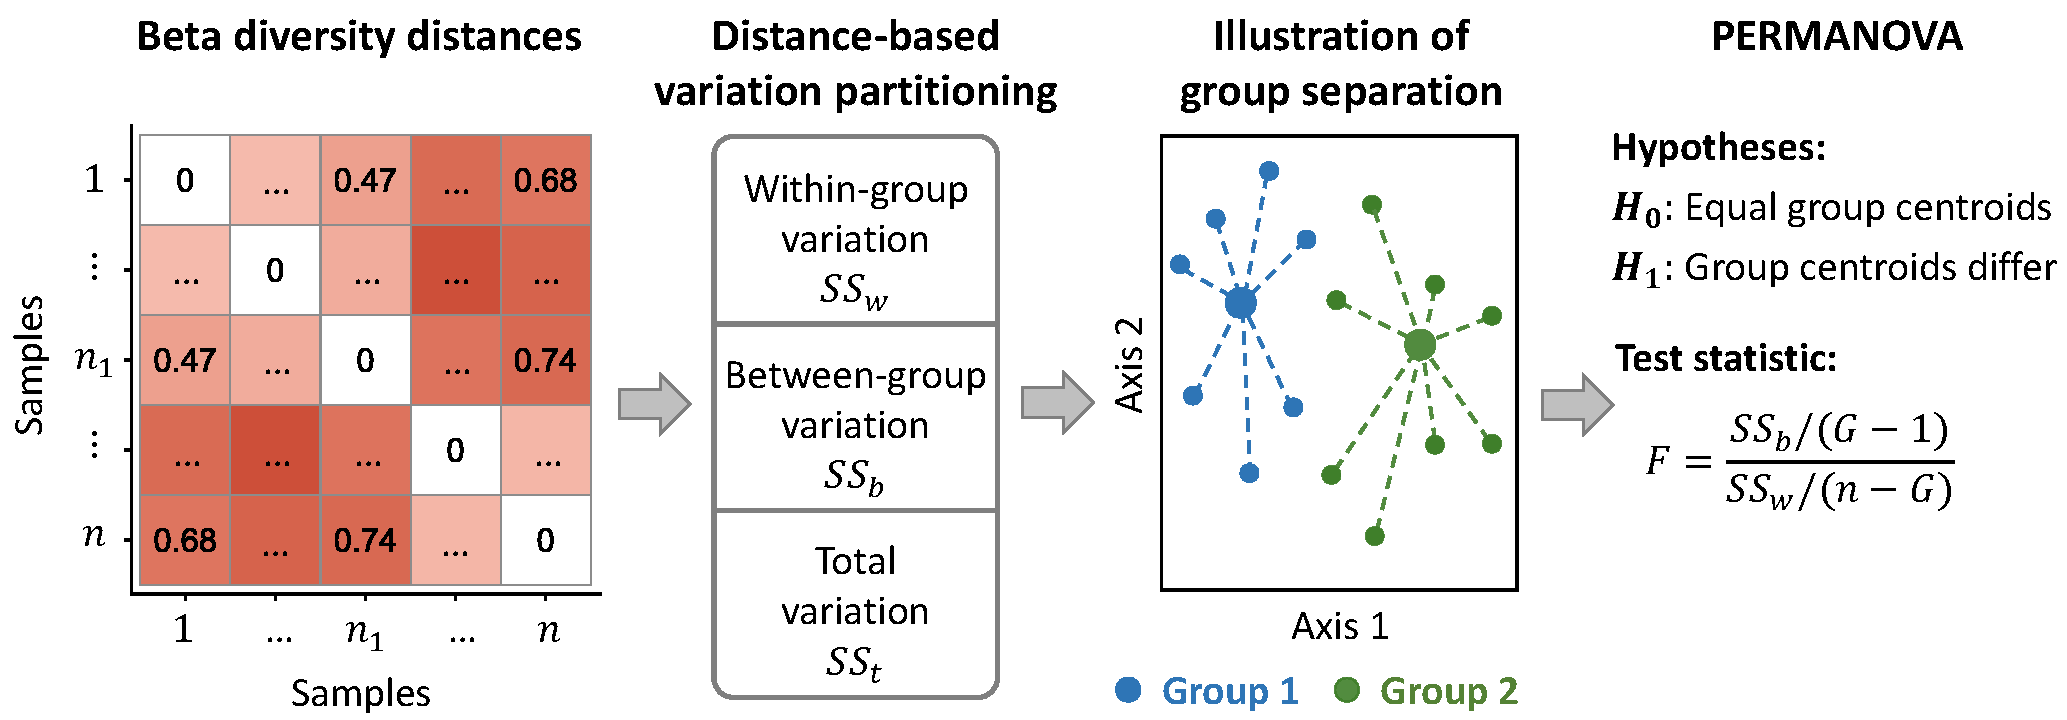
\includegraphics[width=\textwidth]{../ch03_community_level/overview_figures/overview_PERMANOVA.pdf}
	\caption{\textbf{Overview of PERMANOVA for between-sample diversity analysis.} A sample-by-sample beta-diversity distance matrix is used to partition total variation into between-group and within-group components. The resulting pseudo-$F$ statistic compares the relative magnitude of between-group to within-group variation and is evaluated by permutation of group labels. The ordination panel provides a two-dimensional illustration of group separation; PERMANOVA itself uses the full distance-based representation rather than only the displayed axes.}
	\label{fig:3community:overview_permanova}
\end{figure}


Ordination provides a visual summary of between-sample dissimilarities, but formal assessment of group differences requires statistical testing. Figure~\ref{fig:3community:overview_permanova} summarizes the main idea of permutational multivariate analysis of variance (PERMANOVA): a beta-diversity distance matrix is decomposed into within-group and between-group variation, and the resulting pseudo-$F$ statistic is evaluated against a permutation-based null distribution. PERMANOVA was originally proposed by \citet{anderson2001new} and is widely used for distance-based inference in ecological community analysis \citep{anderson2013permanova,legendre2012numerical}. It is commonly interpreted as testing whether predefined groups differ in their centroids within the multivariate representation induced by a chosen dissimilarity measure.

Several distance-based tests have been proposed for ecological community data, including analysis of similarities (ANOSIM) \citep{clarke1993nonparametric}, the Mantel test \citep{mantel1967detection}, multi-response permutation procedures \citep{mielke2001permutation}, and PERMANOVA \citep{anderson2001new}. These methods differ in the hypotheses they target and in their sensitivity to the structure of the distance matrix. 
PERMANOVA is widely used in microbiome studies because it can accommodate a broad class of dissimilarity measures, continuous and categorical covariates, and multi-factor study designs through a regression-type model formula \citep{kers2022power}. In contrast to purely rank-based or pairwise procedures, PERMANOVA partitions variation in the distance matrix into components attributable to explanatory variables and residual variation, yielding an $R^2$-type effect size in addition to a permutation-based $p$-value. For Euclidean distances, the group centroids correspond to arithmetic means of the sample coordinates. For general dissimilarities, the same idea is formulated through the distance-based representation underlying the sums-of-squares decomposition.

Let $\mathbf{D}=(d_{kl})$ denote the dissimilarity matrix between $n$ samples, and let $g_k\in\{1,\ldots,G\}$ denote the group assignment of sample $k$. PERMANOVA expresses the total variation represented by the dissimilarity matrix as a sum of squares and partitions this variation into between-group and within-group components \citep{anderson2001new}. In the one-way case, this yields a pseudo-$F$ statistic of the form
\begin{equation}
F_{\mathrm{PERM}}=\frac{\mathrm{SS}_{\mathrm{b}}/(G-1)}{\mathrm{SS}_{\mathrm{w}}/(n-G)},
\end{equation}
where $\mathrm{SS}_{\mathrm{b}}$ denotes the variation explained by differences between group centroids and $\mathrm{SS}_{\mathrm{w}}$ denotes the residual within-group variation. For more general models, the same principle can be extended by partitioning sums of squares according to explanatory variables, analogous to the analysis of variance for univariate responses \citep{mcardle2001fitting,anderson2001new}.

Because the sampling distribution of $F_{\mathrm{PERM}}$ is generally not available analytically, significance is assessed by permutation. Under the null hypothesis of no association between community composition and the variable of interest, the sample labels are exchangeable according to the chosen permutation scheme. The pseudo-$F$ statistic is recomputed for permuted label assignments, and the observed statistic is compared with the resulting permutation distribution. The empirical permutation $p$-value is then obtained as
\begin{equation}
p_{\mathrm{emp}}=\frac{1+\sum_{b=1}^B I(F_b^\ast\geq F_{\mathrm{obs}})}{1+B},
\end{equation}
where $F_{\mathrm{obs}}$ denotes the observed pseudo-$F$ statistic and $F_b^\ast$ the statistic obtained from the $b$-th permutation. The addition of one to numerator and denominator avoids zero permutation $p$-values and corresponds to the convention discussed in Chapter~\ref{ch:permapprox}.

The interpretation of PERMANOVA depends on the dissimilarity measure used as input. Applying PERMANOVA to Bray--Curtis dissimilarities tests for a group effect in the distance-based representation of relative abundance profiles. Applying it to Aitchison distances tests for group differences in the corresponding log-ratio representation. In sparse microbiome data, this interpretation is conditional on the preprocessing used before CLR transformation, including filtering, normalization to a common compositional scale, and zero replacement. Thus, PERMANOVA does not test a universal notion of ``community difference'', but a difference defined by the geometry induced by the selected distance measure. This is important because different distances emphasize different aspects of the data, as discussed in the previous subsections.

A well-known limitation of PERMANOVA is that significant results may reflect differences in group centroids, differences in within-group dispersion, or a combination of both \citep{anderson2006distance,warton2012distance}. In univariate terms, this is analogous to the difficulty of distinguishing a difference in means from a difference in variances when both affect the test statistic. PERMANOVA results should therefore be interpreted together with ordination plots and, where relevant, with tests for homogeneity of multivariate dispersion such as PERMDISP \citep{anderson2006distance}. This is particularly important in unbalanced designs, where heterogeneity of dispersion can affect type I error and interpretation \citep{anderson2013permanova}. This motivates the explicit assessment of community dispersion in the following subsection.

In R, PERMANOVA is widely applied using the \texttt{adonis2} function from the \texttt{vegan} package \citep{oksanen2024vegan}. The \texttt{adonis2} implementation supports formula-based models, different types of sums of squares, and restricted permutation schemes, making it suitable for ecological and microbiome study designs. Computationally efficient implementations such as \texttt{fast.adonis} have been proposed for larger microbiome data sets and produce results consistent with \texttt{adonis} and \texttt{adonis2} for corresponding PERMANOVA quantities \citep{li2022fastadonis}. In the PASTURE application in Chapter~\ref{ch:application}, we use \texttt{adonis2} because \texttt{fast.adonis} is not needed due to the low dimensionality of the data. The analysis is performed for both beta-diversity representations introduced above, namely Bray--Curtis dissimilarities on relative abundance profiles and Aitchison distances after normalization, multiplicative replacement, and CLR transformation. Since PERMANOVA relies on permutation-based inference, we additionally use the \texttt{permApprox} workflow introduced in Chapter~\ref{ch:permapprox} to assess whether the resulting permutation $p$-values can be refined by tail approximation.


%====================================
\subsection{Community dispersion}
\label{sec:3community:between:dispersion}
%====================================

The between-sample dissimilarities introduced above can be used not only to assess differences between groups, but also to quantify heterogeneity within groups. While PERMANOVA focuses on differences between group centroids in the space induced by a dissimilarity measure, community dispersion describes how strongly samples vary around their corresponding group centroid. It can therefore be interpreted as a multivariate analogue of within-group variance \citep{anderson2006distance}.

Let $\mathbf{D}=(d_{kl})$ denote a dissimilarity matrix between samples and let $g_k\in\{1,\ldots,G\}$ denote the group assignment of sample $k$. For a group $g$, let $\mathbf{z}_k$ denote the coordinate representation of sample $k$ obtained from the chosen dissimilarity matrix, for example through principal coordinates analysis. The group centroid is then given by the average coordinate vector
\begin{equation}
	\bar{\mathbf{z}}_g=\frac{1}{n_g}\sum_{k:g_k=g} \mathbf{z}_k.
\end{equation}
The dispersion of sample $k$ is defined as its distance to the centroid of its group in this coordinate representation,
\begin{equation}
	\delta_k=\left\|\mathbf{z}_k-\bar{\mathbf{z}}_{g_k}\right\|_2.
\end{equation}
where $n_g$ denotes the number of samples in group $g$. Larger values of $\Delta_g$ indicate greater within-group heterogeneity in microbial community composition, whereas smaller values indicate that samples within the group are more similar to each other.

For Euclidean distances, such as the Aitchison distance, the centroid corresponds to the arithmetic mean of the transformed sample coordinates within the group. For non-Euclidean dissimilarities, such as Bray--Curtis dissimilarity, the same idea is implemented through a coordinate representation, typically principal coordinates analysis. In that case, distances to group centroids or spatial medians are computed in the coordinate space that represents the original dissimilarities as closely as possible \citep{anderson2006distance}. Consequently, dispersion estimates should always be interpreted relative to the chosen dissimilarity measure and data representation.

Differences in community dispersion can be assessed using distance-based tests for homogeneity of multivariate dispersions, commonly referred to as PERMDISP \citep{anderson2006distance}. The corresponding null hypothesis is
\begin{equation}
H_0:\Delta_1=\Delta_2=\cdots=\Delta_G.
\end{equation}
In practice, the sample-wise distances $\delta_k$ are treated as univariate responses and compared between groups using an analysis-of-variance type statistic. Significance is commonly assessed using permutation-based procedures. In R, this approach is implemented in the \texttt{betadisper} function of the \texttt{vegan} package, with permutation-based testing available through \texttt{permutest.betadisper} \citep{oksanen2024vegan}.

Community dispersion captures a different aspect of group structure than centroid location. A group with larger dispersion does not necessarily have a different average community composition, but may exhibit greater between-individual variability. In microbiome studies, increased dispersion indicates greater between-individual heterogeneity in community composition and may be consistent with less stable community structures. At the same time, dispersion is important for the interpretation of PERMANOVA: if groups differ in their within-group dispersion, a significant PERMANOVA result may reflect heterogeneity differences rather than, or in addition to, differences in group centroids \citep{anderson2006distance,warton2012distance}. Reporting PERMDISP alongside PERMANOVA therefore helps assess whether differences in within-group dispersion accompany a PERMANOVA finding and supports a more careful interpretation of distance-based microbiome comparisons.

In the PASTURE application in Chapter~\ref{ch:application}, community dispersion is assessed for the same beta-diversity representations used in PERMANOVA, namely Bray--Curtis dissimilarities on relative abundance profiles and Aitchison distances after normalization, multiplicative replacement, and CLR transformation. This allows within-group heterogeneity to be compared on both the ecological relative-abundance scale and the log-ratio scale. Since PERMDISP is also commonly assessed by permutation, we additionally evaluate whether the resulting permutation $p$-values can be refined using the \texttt{permApprox} workflow introduced in Chapter~\ref{ch:permapprox}.

%%%%%%%%%%%%%%%%%%%%%%%%%%%%%%%%%%%%%
\section{Regression models for compositional responses}
\label{sec:3community:regression}
%%%%%%%%%%%%%%%%%%%%%%%%%%%%%%%%%%%%%

\begin{figure}[!ht]
\centering
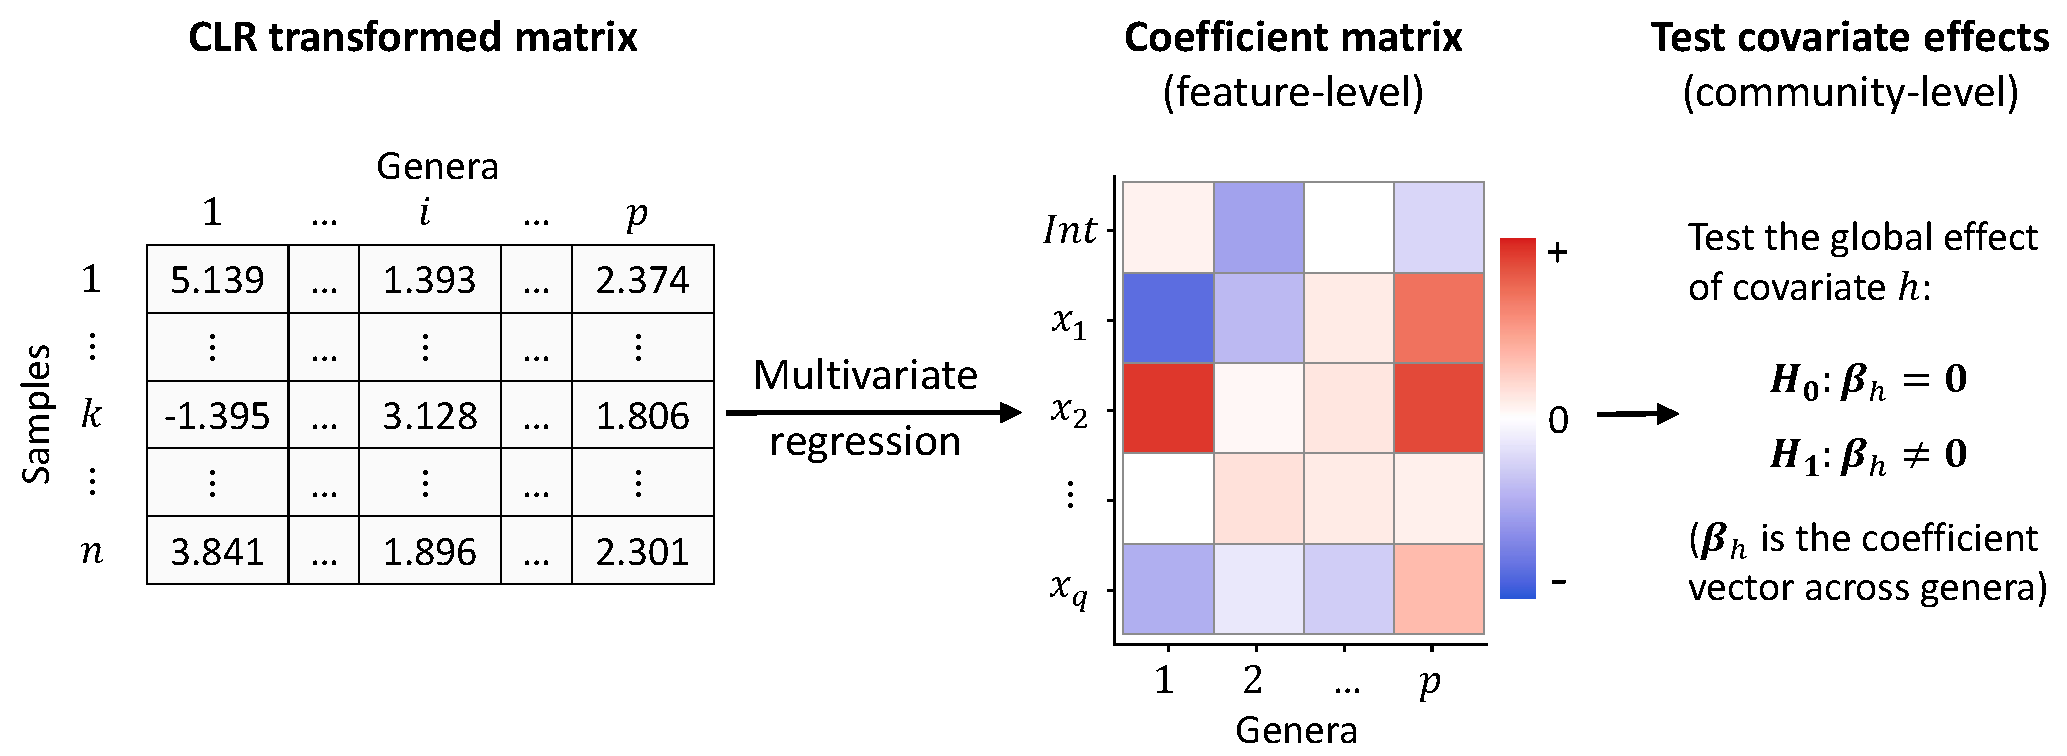
\includegraphics[width=\textwidth]{../ch03_community_level/overview_figures/overview_regression.pdf}
\caption{\textbf{Overview of CLR-based multivariate regression.} A CLR-transformed microbiome count matrix is modeled jointly as a multivariate response using sample-level covariates. The fitted model yields a coefficient matrix with one coefficient vector across taxa for each covariate. Community-level inference tests whether the coefficient vector associated with covariate $h$ is equal to the zero vector, corresponding to no association between that covariate and the overall microbial composition.}
\label{fig:community:regression:overview}
\end{figure}

Regression models provide a model-based perspective on community-level microbiome analysis. Instead of summarizing each sample by a single diversity value or representing between-sample differences only through a dissimilarity matrix, the microbial profile itself can be treated as a multivariate response. This makes it possible to ask whether sample-level covariates are associated with systematic shifts in the microbial composition as a whole. In the context of this thesis, such models are used as global community-level analyses: the main inferential target is not a single taxon-specific coefficient, but the joint covariate effect across the transformed microbial profile.

Figure~\ref{fig:community:regression:overview} summarizes this regression perspective. The following subsections first place the approach in the broader landscape of models for microbial compositions and then introduce the CLR-based multivariate regression model used in this thesis.

%====================================
\subsection{Approaches for modeling microbial compositions}
\label{sec:3community:regression:approaches}
%====================================

Regression models with microbial compositions as response variables can be formulated in different ways, depending on how the simplex constraint, sequencing variability, sparsity, high dimensionality, and covariance between taxa are represented. A first class of approaches models the composition directly by using distributions defined on the simplex. Dirichlet regression is a classical example and provides a generalized linear model-type framework for compositional responses \citep{maier2014dirichletreg}. Such models respect the constant-sum constraint by construction, but the Dirichlet distribution imposes a restrictive mean--variance relationship and negative dependence structure, which can be limiting for sparse and overdispersed microbiome data.

\newpage
A second class of approaches models the observed count vector while introducing a latent compositional layer. Logistic-normal multinomial regression, for example, combines multinomial sampling of sequencing counts with latent log-ratio variables whose mean depends on sample-level covariates \citep{xia2013logistic}. This is attractive for microbiome data because it can represent sampling variability, overdispersion, sampling zeros, and a more flexible covariance structure between taxa. However, such hierarchical count models typically require stronger distributional assumptions and more involved estimation than transformation-based approaches.

A third approach is to transform the microbial composition into log-ratio coordinates and then use regression ideas in the transformed space. This strategy is closely aligned with compositional data analysis, where log-ratio transformations are used to represent relative information in Euclidean coordinates \citep{aitchison1986statistical,gloor2017microbiome,quinn2019field}. Related microbiome methods include linear models on centered log-ratio transformed taxa, as used for example in LinDA for differential abundance analysis \citep{zhou2022linda}, and the LDM-clr framework, which extends the linear decomposition model \citep{hu2020testing} to centered-log-ratio-transformed microbiome data and provides both global and taxon-level tests \citep{hu2023compositional}.

In genuinely high-dimensional microbiome settings with $p\gg n$, unrestricted multivariate regression models are usually not appropriate without additional structural assumptions. The coefficient matrix then contains many parameters relative to the available sample size, and classical multivariate inference may require covariance matrices that are singular or unstable. A common strategy is therefore to impose low-rank, sparse, or latent-factor structure on the multivariate response model. Multivariate reduced-rank regression \citep{reinsel2022multivariate} assumes that the coefficient matrix has low rank, so that covariate effects on many taxa are represented through a smaller number of latent response directions. Sparse reduced-rank regression further combines this low-dimensional structure with sparsity, allowing only selected covariates or response coordinates to contribute to the dominant association patterns. For microbiome count data, count-based variants are particularly relevant because they can account for overdispersion and discreteness directly. For example, \citet{mishra2022negative} proposed negative-binomial reduced-rank regression and negative-binomial co-sparse factor regression to jointly model overdispersed amplicon sequencing counts using low-rank or sparse factor structure. More generally, latent factor models and regularized multivariate regression models provide a principled way to address high-dimensional, sparse, and dependent microbial responses. These approaches address an additional aspect of the regression problem compared with the transformation-based regression considered below: they regularize or factorize the high-dimensional response structure, whereas the model used in this thesis primarily addresses compositionality by working in log-ratio coordinates.

In the present chapter, we follow the transformation-based perspective, but use it as a community-level regression analysis. This interpretation is appropriate when inference focuses on joint covariate effects across the complete microbial profile rather than on separate taxon-specific coefficients, and when the response dimension remains moderate relative to the sample size after aggregation and filtering. This is the case in the PASTURE application in Section~\ref{sec:7app:regression}, where the analysis is conducted at genus level after prevalence filtering. The approach should therefore not be understood as a general solution to high-dimensional microbial response regression, but as a pragmatic model-based approach for studying covariate effects on microbial compositions in moderate-dimensional settings.

%====================================
\subsection{CLR-based multivariate regression}
\label{sec:3community:regression:clr_model}
%====================================

Following the general strategy introduced in Chapter~\ref{ch:microbiome}, we use a CLR-based representation when the microbial composition enters the model as a multivariate response. This avoids formulating regression models directly on raw counts or untransformed relative abundances, whose components carry relative rather than absolute information and may be affected by closure-induced dependencies and library size variation \citep{aitchison1986statistical,gloor2017microbiome,quinn2019field}. 

Using a CLR transformation raises again the question of zero handling. In this regression setting, the transformed taxon profiles are the response variables, so artificial changes in their marginal distributions can directly affect coefficient estimation and testing. Following the preprocessing strategy described in Section~\ref{sec:2micro:preprocessing_choices_thesis}, count data are first brought to a common compositional scale before zero replacement. We then use multiplicative replacement followed by the standard CLR transformation, unless a method-specific alternative is explicitly required. Multiplicative replacement yields strictly positive compositions while preserving ratios among originally non-zero components. This is preferable here to global offset addition, which changes ratios among observed components and can therefore alter the transformed response values before the regression model is fitted. 
Let $\mathbf{x}_k^\ast$ denote the normalized and multiplicatively replaced composition obtained from sample $\mathbf{x}_k$, and define
\begin{equation}
\mathbf{y}_k=\operatorname{CLR}\left(\mathbf{x}_k^\ast\right)\in\mathbb{R}^p
\end{equation}
as the CLR-transformed microbial profile of sample $k$. A multivariate regression model for the transformed composition can then be written as
\begin{equation}
\mathbf{y}_k = \boldsymbol{\beta}_0 + \sum_{h=1}^q w_{kh}\boldsymbol{\beta}_h + \boldsymbol{\varepsilon}_k,
\end{equation}
where $\mathbf{w}_k=(w_{k1},\ldots,w_{kq})^\top$ denotes the vector of $q$ sample-level covariates for sample $k$, $\boldsymbol{\beta}_0\in\mathbb{R}^p$ is an intercept vector, $\boldsymbol{\beta}_h\in\mathbb{R}^p$ denotes the multivariate effect of covariate $h$ across the CLR coordinates, and $\boldsymbol{\varepsilon}_k\in\mathbb{R}^p$ denotes the residual vector. Equivalently, the coefficient vectors can be collected in the coefficient matrix $\mathbf{B}=(\boldsymbol{\beta}_1,\ldots,\boldsymbol{\beta}_q)^\top\in\mathbb{R}^{q\times p}$, yielding the compact representation
\begin{equation}
\mathbf{y}_k = \boldsymbol{\beta}_0 + \mathbf{B}^\top \mathbf{w}_k + \boldsymbol{\varepsilon}_k.
\end{equation}
In this representation, row $h$ of $\mathbf{B}$ contains the coefficients describing the effect of covariate $h$ across all CLR coordinates, whereas column $i$ contains the coefficients associated with CLR coordinate $i$ across all covariates. 

The coefficient interpretation follows the CLR scale on which the response is modeled. A positive coefficient for CLR coordinate $i$ indicates that, conditional on the other covariates, taxon $i$ tends to increase relative to the sample-wise geometric mean as the corresponding covariate increases. Since CLR coordinates express each taxon relative to the sample-wise geometric mean, coefficients describe changes in the relative position of taxa within the microbial composition. They should therefore be understood as effects on the log-ratio representation of the community rather than as marginal effects on absolute or raw relative abundances. 

For the purposes of this chapter, the main inferential target is not an individual coefficient but the covariate-specific effect vector $\boldsymbol{\beta}_h$. Testing whether $\boldsymbol{\beta}_h=\mathbf{0}$ asks whether covariate $h$ is associated with the microbial composition as a whole. This distinguishes compositional-response regression from feature-level regression, where the primary focus lies on taxon-specific effects. At the same time, inference for the coefficient matrix $\mathbf{B}$ is non-trivial because microbiome data are high-dimensional and the CLR coordinates are statistically dependent. The question of how covariate effects are tested is therefore considered separately in the next subsection.

%====================================
\subsection{Testing covariate effects}
\label{sec:3community:regression:testing}
%====================================

In compositional-response regression, the main inferential question is whether a sample-level covariate is associated with the microbial composition as a whole. For covariate $h$, this corresponds to the global null hypothesis
\begin{equation}
H_0:\boldsymbol{\beta}_h=\mathbf{0},
\end{equation}
where $\boldsymbol{\beta}_h\in\mathbb{R}^p$ denotes the vector of coefficients for covariate $h$ across all CLR coordinates. Rejecting this null hypothesis indicates that the covariate is associated with a multivariate shift in the transformed microbial composition. The test is therefore community-level in its interpretation, even though the coefficient vector contains taxon-specific components.

Classical multivariate linear models are commonly tested using MANOVA-type statistics, such as Wilks' lambda, Pillai's trace, the Hotelling--Lawley trace, or Roy's largest root \citep{rencher2002methods}. These statistics compare the variation explained by a covariate with the residual variation in the multivariate response. In matrix notation, let $\mathbf{Y}\in\mathbb{R}^{n\times p}$ denote the matrix of CLR-transformed microbial profiles and let $\mathbf{W}\in\mathbb{R}^{n\times q}$ denote the design matrix of sample-level covariates. Testing a covariate can be formulated by comparing a full model including the covariate with a reduced model in which the covariate is omitted. The difference in fitted values or residual sums of squares then quantifies the contribution of that covariate to explaining variation in the transformed microbial composition.

However, the assumptions underlying classical MANOVA are often difficult to justify for microbiome data. The CLR coordinates are statistically dependent because they are constrained to sum to zero, and microbiome data are typically sparse and high-dimensional, with the number of taxa often comparable to or larger than the number of samples \citep{aitchison1986statistical,gloor2017microbiome,xia2024applied}. For CLR-transformed responses, the residual covariance matrix is structurally singular because the coordinates sum to zero. High dimensionality can further make covariance estimation unstable, and normality assumptions for transformed microbial profiles are at best approximate. Classical asymptotic MANOVA approximations should therefore be interpreted with caution in microbiome applications, especially when $p$ is not small relative to $n$ \citep{chen2010twosample}.

A permutation-based alternative is to use a global test statistic for the covariate effect and approximate its null distribution under an appropriate exchangeability scheme \citep{freedman1983nonstochastic,winkler2014permutation}. Related microbiome-specific approaches include the linear decomposition model and its CLR-based extension, which use regression-type formulations to obtain community-level tests together with taxon-level information \citep{hu2020testing,hu2023compositional}. One possible statistic is the reduction in multivariate residual sum of squares when covariate $h$ is added to the model,
\begin{equation}
t_h=\mathrm{RSS}_{\mathrm{red},h}-\mathrm{RSS}_{\mathrm{full}},
\end{equation}
where the residual sum of squares is computed over all samples and CLR coordinates, for example as the squared Frobenius norm of the residual matrix,
\begin{equation}
\mathrm{RSS}=\|\mathbf{Y}-\widehat{\mathbf{Y}}\|_F^2.
\end{equation}
Here, $\mathrm{RSS}_{\mathrm{full}}$ denotes the residual sum of squares of the full multivariate model and $\mathrm{RSS}_{\mathrm{red},h}$ denotes the residual sum of squares of the model without covariate $h$. Larger values of $t_h$ indicate that the covariate explains more variation in the CLR-transformed microbial profile. This construction is analogous to comparing nested regression models, but the null distribution is obtained empirically rather than from a parametric approximation.

The empirical permutation $p$-value is then computed by comparing the observed statistic $t_{h,\mathrm{obs}}$ with the statistics $t_{hb}^\ast$, $b=1,\ldots,B$, obtained from permuted data:
\begin{equation}
p_{\mathrm{emp},h}=\frac{1+\sum_{b=1}^B I(t_{hb}^\ast\geq t_{h,\mathrm{obs}})}{1+B}.
\end{equation}
This formulation follows the general permutation-testing principle discussed in Chapter~\ref{ch:permapprox}. It is attractive in the present setting because it avoids relying on a parametric null distribution for a high-dimensional multivariate response and can be applied with the same transformed response matrix used for coefficient estimation.

In the PASTURE application in Chapter~\ref{ch:application}, compositional-response regression is used as an additional community-level analysis for the selected birth-related covariates. The focus is on the global covariate tests $H_0:\boldsymbol{\beta}_h=\mathbf{0}$, not on interpreting individual taxon-specific coefficients as separate feature-level findings. Since the tests are permutation-based, we also evaluate whether the resulting permutation $p$-values can be refined using the \texttt{permApprox} workflow introduced in Chapter~\ref{ch:permapprox}. This allows the regression-based analysis to be compared with the distance-based PERMANOVA results while retaining the same inferential framework for limited permutation settings.


%%%%%%%%%%%%%%%%%%%%%%%%%%%%%%%%%%%%%
\section{Compositional equivalence}
\label{sec:3community:compositional_equivalence}
%%%%%%%%%%%%%%%%%%%%%%%%%%%%%%%%%%%%%

\begin{figure}[H]
	\centering
	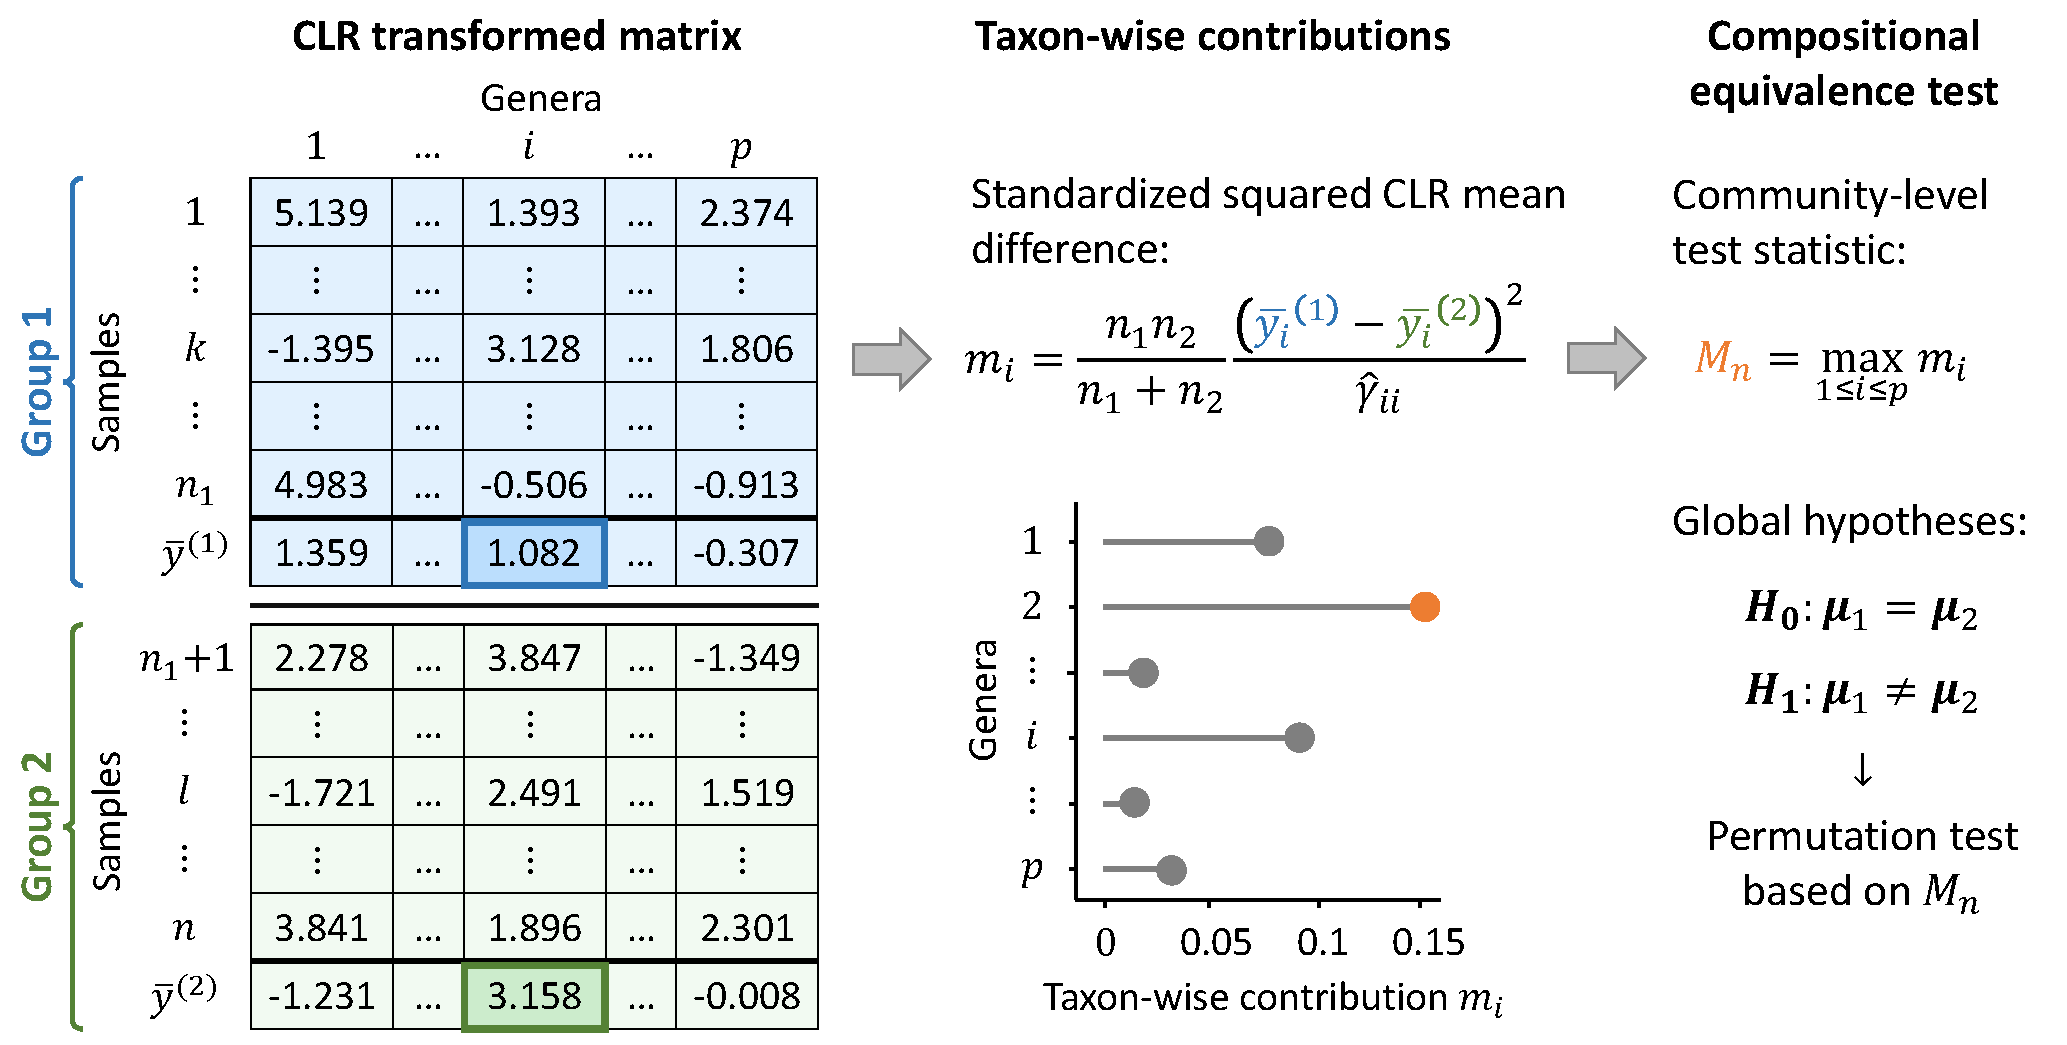
\includegraphics[width=\textwidth]{../ch03_community_level/overview_figures/overview_comp_equivalence.pdf}
	\caption{\textbf{Overview of compositional equivalence testing.} The microbiome data are represented on the CLR scale, and group-specific mean CLR vectors are computed for the two groups. For each taxon, the standardized squared difference between the group means defines a taxon-wise contribution $m_i$. The largest contribution is summarized by the maximum-type statistic $M_n$, which is evaluated using a permutation test of equality between the group mean CLR compositions.}
	\label{fig:3community:overview_comp_equivalence}
\end{figure}

The preceding sections considered community-level summaries from complementary perspectives. Within-sample diversity reduces each microbial profile to a scalar summary, between-sample dissimilarity represents community structure through pairwise distances between samples, and regression models for compositional responses treat the transformed microbial profile as a multivariate outcome. \emph{Compositional equivalence} provides a further perspective at the boundary between community-level and feature-level inference. It is constructed from taxon-specific differences in centered log-ratio coordinates, but these differences are aggregated through a maximum-type statistic, yielding a single global test for the microbial composition. The main steps of the procedure are summarized in Figure~\ref{fig:3community:overview_comp_equivalence}.

%====================================
\subsection{Concept and hypothesis}
\label{sec:3community:comp_equivalence:concept}
%====================================

The idea of compositional equivalence is to compare the average microbial composition between groups while respecting that the observed data contain only relative abundance information. A direct comparison of raw mean count vectors or mean relative abundance vectors would not define an appropriate inferential target, because such comparisons are affected by library size differences and the closure constraint discussed in Chapter~2. Following the compositional data framework, \citet{cao2018twosample} formulate group comparison in log-ratio coordinates. In this thesis, compositional equivalence is computed after total sum normalization, multiplicative replacement of zero counts, and CLR transformation, following the preprocessing strategy described in Section~\ref{sec:2micro:preprocessing_choices_thesis}. The CLR transformation itself was introduced in Section~\ref{sec:2micro:norm:log-ratios}, and its use in the presence of zeros was discussed in Section~\ref{sec:2micro:clr_with_zeros}. Let $\mathbf{y}_k^{(g)}$ denote the resulting CLR representation of the microbial composition of sample $k$ in group $g\in\{1,2\}$. Group differences can then be formulated as differences between the corresponding mean CLR vectors.

The null hypothesis states that the two groups have equal mean log-ratio composition,
\begin{equation}
H_0:\boldsymbol{\mu}_1=\boldsymbol{\mu}_2,
\end{equation}
where $\boldsymbol{\mu}_g=\mathbb{E}\left(\mathbf{y}_k^{(g)}\right)$ denotes the population mean of the CLR-transformed composition in group $g$. Since CLR coordinates are invariant to multiplication of the original composition by a positive constant, this hypothesis is formulated in terms of relative microbial composition rather than absolute microbial load. Thus, compositional equivalence is a global statement about equality of mean relative composition in log-ratio space. Deviations from this null hypothesis indicate that the groups differ in at least one component of their mean CLR composition, but not necessarily that they differ in total microbial load, which is not identified from standard sequencing data.

%====================================
\subsection{Maximum-type test statistic}
\label{sec:3community:comp_equivalence:statistic}
%====================================

A natural test statistic for this hypothesis compares the sample mean vectors in CLR space. Let
\begin{equation}
	\bar{\mathbf{y}}^{(g)} = 
	\frac{1}{n_g}
	\sum_{k=1}^{n_g}
	\mathbf{y}_k^{(g)}
\end{equation}
denote the sample mean CLR vector in group $g$, and let $\hat{\gamma}_{ii}$ denote the pooled within-group variance estimate of CLR coordinate $i$. For each taxon $i$, the standardized squared difference between the group-specific sample means is defined as
\begin{equation}
	m_i = \frac{n_1n_2}{n_1+n_2} \frac{\left(\bar{y}_i^{(1)}-\bar{y}_i^{(2)}\right)^2}
	{\hat{\gamma}_{ii}}.
	\label{eq:3community:comp_equivalence:coordinate_contribution}
\end{equation}
The statistic proposed by \citet{cao2018twosample} is then obtained by taking the maximum over all coordinate-wise contributions,
\begin{equation}
	M_n = \max_{1\leq i\leq p} m_i.
	\label{eq:3community:comp_equivalence:maximum_statistic}
\end{equation}
Thus, the procedure evaluates standardized differences between group-specific CLR means for all taxa and summarizes the largest contribution in a single global statistic. This maximum-type construction is motivated by sparse alternatives, in which differences between groups are concentrated in only a small number of taxa. In such settings, statistics that aggregate contributions across many coordinates may dilute the signal, whereas a maximum statistic is sensitive to the largest standardized deviation. Nevertheless, the inferential target remains global: the test assesses whether the mean CLR compositions differ between groups, rather than identifying individual taxa responsible for a potential difference.


%====================================
\subsection{Permutation-based inference and application}
\label{sec:3community:comp_equivalence:permutation}
%====================================

In microbiome applications, randomization-based inference provides an attractive alternative to asymptotic approximations. \citet{sommer2022randomizationbased} considered a related maximum-type test within a randomization-based causal-inference framework. They emphasized that, because sequencing data are compositional, a change in the observed abundance of one taxon necessarily affects the observed counts of other taxa, even when these taxa have no causal role. Their approach therefore applies a CLR transformation before comparing group-specific mean log-ratio compositions and uses a maximum-type statistic based on standardized differences between group mean CLR coordinates.

In this thesis, $M_n$ is used as a permutation test statistic rather than being evaluated through an asymptotic approximation. Since total sum scaling, multiplicative zero replacement, and CLR transformation are applied sample-wise and independently of the group labels, the transformed data are kept fixed during the permutation procedure. Group labels are then permuted repeatedly, and the statistic $M_n^\ast$ is recomputed for each permuted labeling, including the corresponding group-specific mean vectors and pooled within-group coordinate variances. The observed statistic is compared with the resulting permutation distribution. For $B$ permutations, the empirical permutation $p$-value is computed as
\begin{equation}
	p_{\mathrm{emp}} = \frac{1+\sum_{b=1}^{B} I\left(M_{n,b}^\ast \geq M_n\right)} {B+1}.
	\label{eq:3community:comp_equivalence:empirical_pvalue}
\end{equation}
This procedure is valid when samples are exchangeable with respect to the group labels under the null hypothesis. More complex study designs may require restricted or covariate-adjusted permutation schemes.

The permutation-based formulation is aligned with the general inferential strategy of this thesis and avoids reliance on large-sample approximations whose accuracy may be difficult to assess for sparse, high-dimensional microbiome data. At the same time, it inherits the finite-resolution limitation of permutation testing: with a limited number of permutations, attainable $p$-values lie on a discrete grid. Small empirical $p$-values from the maximum-type test are therefore refined using the \texttt{permApprox} framework developed in Chapter~\ref{ch:permapprox}. In this setting, $M_n$ is treated as the observed right-tailed test statistic, and the permuted values $M_{n,1}^\ast,\ldots,M_{n,B}^\ast$ define the permutation distribution used for tail approximation.

Within the organization of this thesis, compositional equivalence serves as a final community-level comparison that is close to feature-level inference. In contrast to within-sample diversity analysis, it uses the complete transformed microbial profile rather than reducing each sample to a scalar ecological summary. In contrast to PERMANOVA, it is not based on pairwise sample dissimilarities, but on differences between group-specific mean CLR vectors. In contrast to feature-level differential abundance analysis, it does not yield one hypothesis test per taxon, but combines taxon-wise CLR contrasts into a single global test. In the PASTURE application, this makes the method a useful additional analysis for selected two-group contrasts identified in the preceding community-level analyses.

A significant result indicates evidence that the groups differ in their mean log-ratio composition, with particular sensitivity to sparse shifts in CLR coordinates. It does not, by itself, identify the taxa responsible for the difference and does not imply a difference in absolute microbial load. Conversely, a non-significant result should be interpreted as a lack of evidence against equality of mean CLR compositions under the chosen preprocessing strategy and test statistic, rather than as proof of identical microbial communities.
